\documentclass[10pt  ,usenames, dvipsnames]{article}\usepackage[]{graphicx}\usepackage[]{color}
%% maxwidth is the original width if it is less than linewidth
%% otherwise use linewidth (to make sure the graphics do not exceed the margin)
\makeatletter
\def\maxwidth{ %
  \ifdim\Gin@nat@width>\linewidth
    \linewidth
  \else
    \Gin@nat@width
  \fi
}
\makeatother

\definecolor{fgcolor}{rgb}{0.345, 0.345, 0.345}
\newcommand{\hlnum}[1]{\textcolor[rgb]{0.686,0.059,0.569}{#1}}%
\newcommand{\hlstr}[1]{\textcolor[rgb]{0.192,0.494,0.8}{#1}}%
\newcommand{\hlcom}[1]{\textcolor[rgb]{0.678,0.584,0.686}{\textit{#1}}}%
\newcommand{\hlopt}[1]{\textcolor[rgb]{0,0,0}{#1}}%
\newcommand{\hlstd}[1]{\textcolor[rgb]{0.345,0.345,0.345}{#1}}%
\newcommand{\hlkwa}[1]{\textcolor[rgb]{0.161,0.373,0.58}{\textbf{#1}}}%
\newcommand{\hlkwb}[1]{\textcolor[rgb]{0.69,0.353,0.396}{#1}}%
\newcommand{\hlkwc}[1]{\textcolor[rgb]{0.333,0.667,0.333}{#1}}%
\newcommand{\hlkwd}[1]{\textcolor[rgb]{0.737,0.353,0.396}{\textbf{#1}}}%
\let\hlipl\hlkwb

\usepackage{framed}
\makeatletter
\newenvironment{kframe}{%
 \def\at@end@of@kframe{}%
 \ifinner\ifhmode%
  \def\at@end@of@kframe{\end{minipage}}%
  \begin{minipage}{\columnwidth}%
 \fi\fi%
 \def\FrameCommand##1{\hskip\@totalleftmargin \hskip-\fboxsep
 \colorbox{shadecolor}{##1}\hskip-\fboxsep
     % There is no \\@totalrightmargin, so:
     \hskip-\linewidth \hskip-\@totalleftmargin \hskip\columnwidth}%
 \MakeFramed {\advance\hsize-\width
   \@totalleftmargin\z@ \linewidth\hsize
   \@setminipage}}%
 {\par\unskip\endMakeFramed%
 \at@end@of@kframe}
\makeatother

\definecolor{shadecolor}{rgb}{.97, .97, .97}
\definecolor{messagecolor}{rgb}{0, 0, 0}
\definecolor{warningcolor}{rgb}{1, 0, 1}
\definecolor{errorcolor}{rgb}{1, 0, 0}
\newenvironment{knitrout}{}{} % an empty environment to be redefined in TeX

\usepackage{alltt}
\usepackage{graphicx, verbatim}
\usepackage{amsmath}
\usepackage{amssymb}
\usepackage{amscd}
\usepackage{lipsum}
\usepackage{todonotes}
\usepackage[tableposition=top]{caption}
\usepackage{ifthen}
\usepackage[utf8]{inputenc}
\usepackage{graphicx}
\usepackage{caption}
\usepackage{listings}
\usepackage{color}
\setlength{\textwidth}{6.5in} 
\setlength{\textheight}{9in}
\setlength{\oddsidemargin}{0in} 
\setlength{\evensidemargin}{0in}
\setlength{\topmargin}{-1.5cm}
\setlength{\parindent}{0cm}
\usepackage{setspace}
\usepackage{float}
\usepackage{amssymb}
\usepackage[utf8]{inputenc}
\usepackage{fancyhdr}
\usepackage{tabularx}
\usepackage{lmodern} % for bold teletype font
\usepackage{minted}

\usepackage{hyperref}
\hypersetup{
  colorlinks   = true, %Colours links instead of ugly boxes
  urlcolor     = blue, %Colour for external hyperlinks
  linkcolor    = blue, %Colour of internal links
  citecolor   = red %Colour of citations
}

%\fancyhf{}
\rfoot{Andrew Tait \thepage}
\singlespacing
\usepackage[affil-it]{authblk} 
\usepackage{etoolbox}
\usepackage{lmodern}

% Notice the following package, it will help you cite papers
\usepackage[backend=bibtex ,sorting=none]{biblatex}
\bibliography{references}
\IfFileExists{upquote.sty}{\usepackage{upquote}}{}
\begin{document}


\title{\LARGE Coursework  \\ Data Science Development (CMM535)}

\author{Andrew Tait, \textit{\href{1504693@rgu.ac.uk}{1504693@rgu.ac.uk}}}
\maketitle
% \begin{flushleft} \today \end{flushleft} 
\noindent\rule{16cm}{0.4pt}
%\underline{\hspace{3cm}
\ \\
%\thispagestyle{empty}



\section {Data Exploration}



\subsection{Dataset Choice}
The dataset that has been chosen for this part of the coursework is Mushroom. This is available on the UCI repository. The set was chosen because of it's adequate instance size and number of attributes.

.


\subsection{Problem Statement and Data Exploration}


The main purpose of the Mushroom dataset is to identify which characteristics (attributes) determine if a particular mushroom species is editable or poisonous.

Therefore the aim of this assignment is to build a predictive model to predict if a certain type of Mushroom is ediable or not.


To start off the data explortation I will first import the required librarys.

\begin{knitrout}
\definecolor{shadecolor}{rgb}{0.969, 0.969, 0.969}\color{fgcolor}\begin{kframe}
\begin{alltt}
\hlcom{#Import packages}
\hlkwd{library}\hlstd{(randomForest)}
\hlkwd{library}\hlstd{(e1071)}
\hlkwd{library}\hlstd{(caret)}
\hlkwd{library}\hlstd{(ggplot2)}
\hlkwd{library}\hlstd{(gridExtra)}
\hlkwd{library}\hlstd{(caret)}
\hlkwd{library}\hlstd{(rpart.plot)}
\hlkwd{library}\hlstd{(RColorBrewer)}
\hlkwd{library}\hlstd{(plyr)}
\end{alltt}
\end{kframe}
\end{knitrout}




Then set the working directory to the Coursework project folder path:
\begin{knitrout}
\definecolor{shadecolor}{rgb}{0.969, 0.969, 0.969}\color{fgcolor}\begin{kframe}
\begin{alltt}
\hlkwd{setwd}\hlstd{(}\hlstr{"~/CMM535 Data Science Development/Coursework/CMM535_Coursework"}\hlstd{)}
\end{alltt}
\end{kframe}
\end{knitrout}



In order to import the dataset, I used a third party helper function, which can be viewed at Figure .
The helper function not only set the attributes names but the instances names as well. Since all the data is represented a single character, it converts them into their string equivalent.


\begin{knitrout}
\definecolor{shadecolor}{rgb}{0.969, 0.969, 0.969}\color{fgcolor}\begin{kframe}
\begin{alltt}
\hlcom{#helper function}
\hlkwd{source}\hlstd{(}\hlstr{'helper_functions.r'}\hlstd{)}

\hlcom{#Import datasets using helper function}

\hlstd{mushroom} \hlkwb{<-} \hlkwd{fetchAndCleanData}\hlstd{()}
\end{alltt}
\end{kframe}
\end{knitrout}





Now that the dataset is imported, it is time to do some data exploration and analysis.

Number of rows in the dataset:

\begin{knitrout}
\definecolor{shadecolor}{rgb}{0.969, 0.969, 0.969}\color{fgcolor}\begin{kframe}
\begin{alltt}
\hlcom{#Number of rows in the dataset}
\hlkwd{nrow}\hlstd{(mushroom)}
\end{alltt}
\end{kframe}
\end{knitrout}


\begin{knitrout}
\definecolor{shadecolor}{rgb}{0.969, 0.969, 0.969}\color{fgcolor}\begin{kframe}
\begin{verbatim}
## [1] 8124
\end{verbatim}
\end{kframe}
\end{knitrout}

Number of columns (features) in the dataset:

\begin{knitrout}
\definecolor{shadecolor}{rgb}{0.969, 0.969, 0.969}\color{fgcolor}\begin{kframe}
\begin{alltt}
\hlkwd{ncol}\hlstd{(mushroom)}
\end{alltt}
\end{kframe}
\end{knitrout}


\begin{knitrout}
\definecolor{shadecolor}{rgb}{0.969, 0.969, 0.969}\color{fgcolor}\begin{kframe}
\begin{verbatim}
## [1] 23
\end{verbatim}
\end{kframe}
\end{knitrout}

Summary of the Mushroom dataset:

\begin{knitrout}
\definecolor{shadecolor}{rgb}{0.969, 0.969, 0.969}\color{fgcolor}\begin{kframe}
\begin{alltt}
\hlcom{#Summary of the Mushroom dataset}
\hlkwd{str}\hlstd{(mushroom)}
\end{alltt}
\end{kframe}
\end{knitrout}


\begin{knitrout}
\definecolor{shadecolor}{rgb}{0.969, 0.969, 0.969}\color{fgcolor}\begin{kframe}
\begin{verbatim}
## 'data.frame':	8124 obs. of  23 variables:
##  $ Edible               : Factor w/ 2 levels "Edible","Poisonous": 2 1 1 2 1 1 1 1 2 1 ...
##  $ CapShape             : Factor w/ 12 levels "b","c","f","k",..: 9 9 7 9 9 9 7 7 9 7 ...
##  $ CapSurface           : Factor w/ 8 levels "f","g","s","y",..: 8 8 8 7 8 7 8 7 7 8 ...
##  $ CapColor             : Factor w/ 20 levels "b","c","e","g",..: 11 20 19 19 14 20 19 19 19 20 ...
##  $ Bruises              : Factor w/ 4 levels "f","t","True",..: 3 3 3 3 4 3 3 3 3 3 ...
##  $ Odor                 : Factor w/ 18 levels "a","c","f","l",..: 17 10 11 17 16 10 10 11 17 10 ...
##  $ GillAttachment       : Factor w/ 6 levels "a","f","Attached",..: 5 5 5 5 5 5 5 5 5 5 ...
##  $ GillSpacing          : Factor w/ 5 levels "c","w","Close",..: 3 3 3 3 4 3 3 3 3 3 ...
##  $ GillSize             : Factor w/ 4 levels "b","n","Broad",..: 4 3 3 4 3 3 3 3 4 3 ...
##  $ GillColor            : Factor w/ 24 levels "b","e","g","h",..: 13 13 14 14 13 14 17 14 20 17 ...
##  $ StalkShape           : Factor w/ 4 levels "e","t","Enlarging",..: 3 3 3 3 4 3 3 3 3 3 ...
##  $ StalkRoot            : Factor w/ 12 levels "?","b","c","e",..: 9 7 7 9 9 7 7 7 9 7 ...
##  $ StalkSurfaceAboveRing: Factor w/ 8 levels "f","k","s","y",..: 8 8 8 8 8 8 8 8 8 8 ...
##  $ StalkSurfaceBelowRing: Factor w/ 8 levels "f","k","s","y",..: 8 8 8 8 8 8 8 8 8 8 ...
##  $ StalkColorAboveRing  : Factor w/ 18 levels "b","c","e","g",..: 17 17 17 17 17 17 17 17 17 17 ...
##  $ StalkColorBelowRing  : Factor w/ 18 levels "b","c","e","g",..: 17 17 17 17 17 17 17 17 17 17 ...
##  $ VeilType             : Factor w/ 3 levels "p","Partial",..: 2 2 2 2 2 2 2 2 2 2 ...
##  $ VeilColor            : Factor w/ 8 levels "n","o","w","y",..: 7 7 7 7 7 7 7 7 7 7 ...
##  $ RingNumber           : Factor w/ 6 levels "n","o","t","None",..: 5 5 5 5 5 5 5 5 5 5 ...
##  $ RingType             : Factor w/ 13 levels "e","f","l","n",..: 11 11 11 11 7 11 11 11 11 11 ...
##  $ SporePrintColor      : Factor w/ 18 levels "b","h","k","n",..: 10 11 11 10 11 10 10 11 10 10 ...
##  $ Population           : Factor w/ 12 levels "a","c","n","s",..: 10 9 9 10 7 9 9 10 11 10 ...
##  $ Habitat              : Factor w/ 14 levels "d","g","l","m",..: 12 8 10 12 8 8 10 10 8 10 ...
\end{verbatim}
\end{kframe}
\end{knitrout}

Now that some basic data exploration is covered, next to inspect the dataset a bit further. Starting with the class (Edible) distribution in the mushroom dataset, see (Figure~\ref{fig1})

\begin{knitrout}
\definecolor{shadecolor}{rgb}{0.969, 0.969, 0.969}\color{fgcolor}\begin{kframe}
\begin{alltt}
\hlcom{#Class Distribution}
\hlkwd{barplot}\hlstd{(}\hlkwd{table}\hlstd{(mushroom}\hlopt{$}\hlstd{Edible))}
\end{alltt}
\end{kframe}
\end{knitrout}
\begin{figure}[H]
\begin{center}
\begin{knitrout}
\definecolor{shadecolor}{rgb}{0.969, 0.969, 0.969}\color{fgcolor}
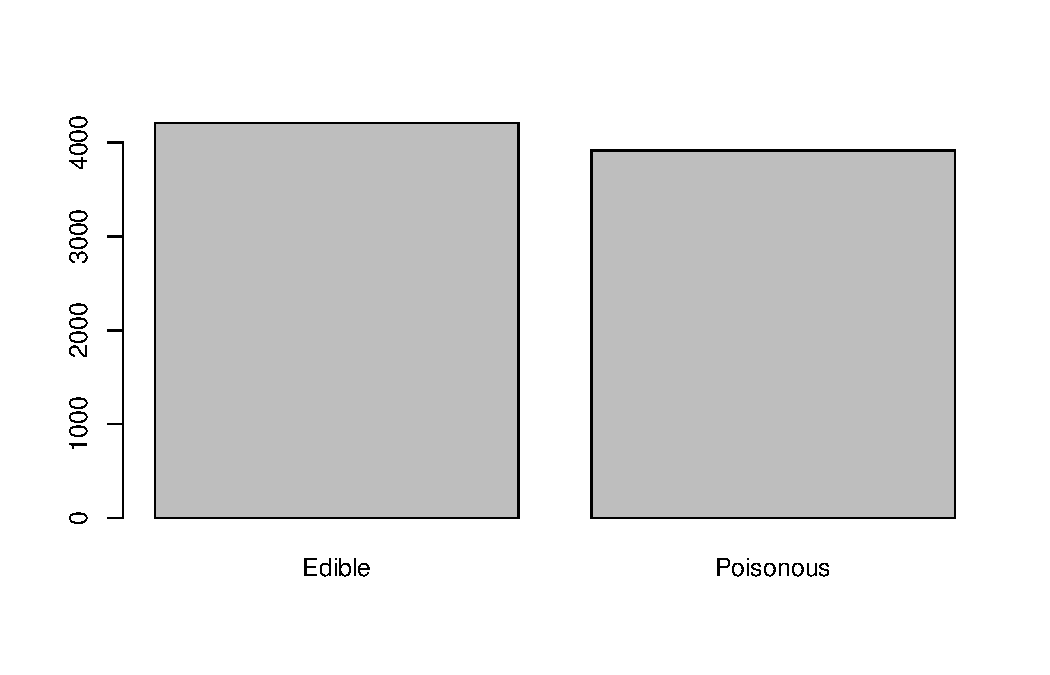
\includegraphics[width=.76\linewidth]{figure/unnamed-chunk-14-1} 

\end{knitrout}
\caption {Barplot of Class Distribution}
\label{fig1}
\end {center}
\end {figure}

Next is to analyse if there is a correlocation between the CapShape and CapSurface of a mushroom and whether it is Edible or Poisonous. Which is shown in the plot ((Figure~\ref{fig2}))below.

\begin{knitrout}
\definecolor{shadecolor}{rgb}{0.969, 0.969, 0.969}\color{fgcolor}\begin{kframe}
\begin{alltt}
\hlcom{#Comparisons of CapShape and CapSurface with Edible or Poisonous}
\hlkwd{ggplot}\hlstd{(mushroom,}\hlkwd{aes}\hlstd{(}\hlkwc{x}\hlstd{=CapShape,} \hlkwc{y}\hlstd{=CapSurface,} \hlkwc{color}\hlstd{=Edible))} \hlopt{+}
                       \hlkwd{geom_jitter}\hlstd{(}\hlkwc{alpha}\hlstd{=}\hlnum{0.3}\hlstd{)} \hlopt{+}
                       \hlkwd{scale_color_manual}\hlstd{(}\hlkwc{breaks} \hlstd{=} \hlkwd{c}\hlstd{(}\hlstr{'Edible'}\hlstd{,}\hlstr{'Poisonous'}\hlstd{),}
                                          \hlkwc{values}\hlstd{=}\hlkwd{c}\hlstd{(}\hlstr{'darkgreen'}\hlstd{,}\hlstr{'red'}\hlstd{))}
\end{alltt}
\end{kframe}
\end{knitrout}

\begin{figure}[H]
\begin{center}
\begin{knitrout}
\definecolor{shadecolor}{rgb}{0.969, 0.969, 0.969}\color{fgcolor}
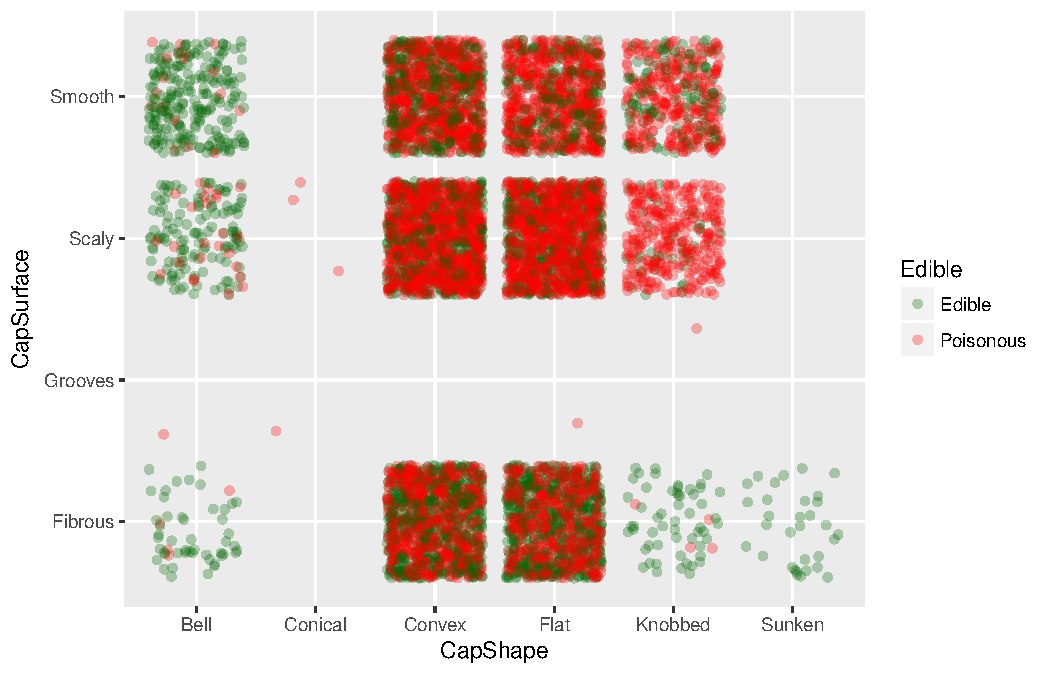
\includegraphics[width=.76\linewidth]{figure/unnamed-chunk-16-1} 

\end{knitrout}
\caption {Comparisons of CapShape and CapSurface with Edible or Poisonous in Mushroom Dataset}
\label{fig2}
\end {center}
\end {figure}

\begin{knitrout}
\definecolor{shadecolor}{rgb}{0.969, 0.969, 0.969}\color{fgcolor}\begin{kframe}
\begin{alltt}
\hlcom{#Comparisons of StalkSurfaceAboveRing and StalkSurfaceBelowRing with Edible or Poisionous}
\hlkwd{ggplot}\hlstd{(mushroom,}\hlkwd{aes}\hlstd{(}\hlkwc{x}\hlstd{=StalkSurfaceAboveRing,} \hlkwc{y}\hlstd{=StalkSurfaceBelowRing,} \hlkwc{color}\hlstd{=Edible))} \hlopt{+}
  \hlkwd{geom_jitter}\hlstd{(}\hlkwc{alpha}\hlstd{=}\hlnum{0.3}\hlstd{)} \hlopt{+}
  \hlkwd{scale_color_manual}\hlstd{(}\hlkwc{breaks} \hlstd{=} \hlkwd{c}\hlstd{(}\hlstr{'Edible'}\hlstd{,}\hlstr{'Poisonous'}\hlstd{),} \hlkwc{values}\hlstd{=}\hlkwd{c}\hlstd{(}\hlstr{'darkgreen'}\hlstd{,}\hlstr{'red'}\hlstd{))}
\end{alltt}
\end{kframe}
\end{knitrout}

\begin{figure}[H]
\begin{center}
\begin{knitrout}
\definecolor{shadecolor}{rgb}{0.969, 0.969, 0.969}\color{fgcolor}
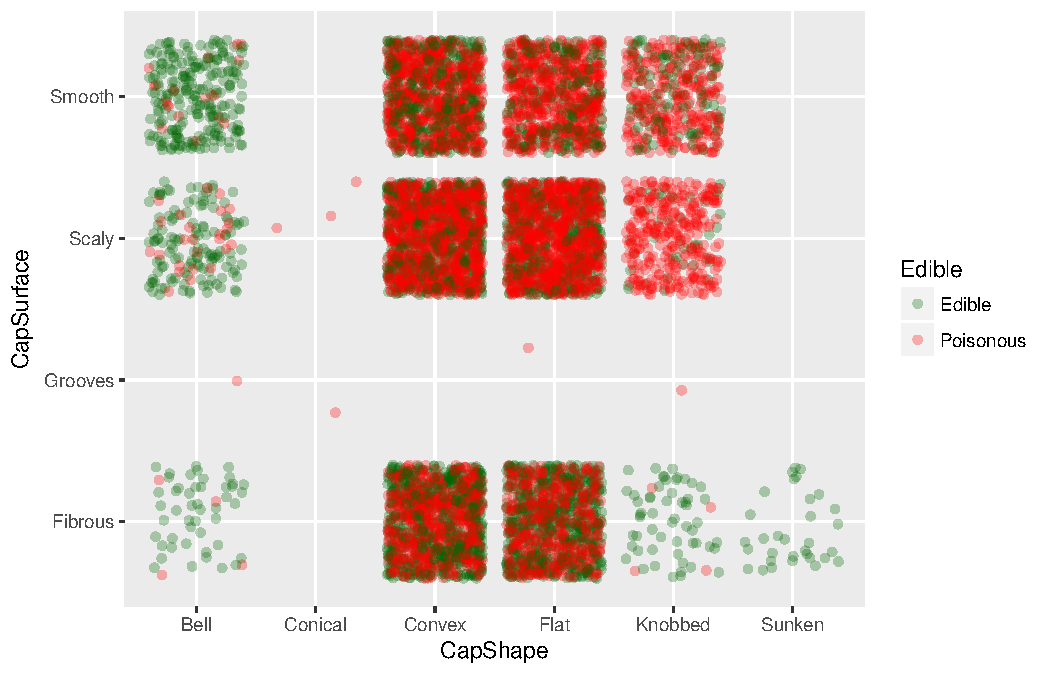
\includegraphics[width=.76\linewidth]{figure/unnamed-chunk-18-1} 

\end{knitrout}
\caption {Comparisons of StalkSurfaceAboveRing and StalkSurfaceBelowRing with Edible or Poisionous}
\label{fig3}
\end {center}
\end {figure}



\clearpage

\subsection {Pre-Processing}

Before the Mushroom dataset can be processed by a classification model(s), some pre-processing is required.

While the helper function should take out all missing values, lets valdiate this before continuing.

\begin{knitrout}
\definecolor{shadecolor}{rgb}{0.969, 0.969, 0.969}\color{fgcolor}\begin{kframe}
\begin{alltt}
\hlcom{#Class Distribution}
\hlkwd{table}\hlstd{(}\hlkwd{complete.cases} \hlstd{(mushroom))}
\end{alltt}
\end{kframe}
\end{knitrout}


\begin{knitrout}
\definecolor{shadecolor}{rgb}{0.969, 0.969, 0.969}\color{fgcolor}\begin{kframe}
\begin{verbatim}
## 
## TRUE 
## 8124
\end{verbatim}
\end{kframe}
\end{knitrout}

As shown above, there is not any missing values in the dataset.

The class (Edible) on the Mushroom dataset is then converted to a factor, this is due to way that certain classification models interact with the class feature of a dataset.


\begin{knitrout}
\definecolor{shadecolor}{rgb}{0.969, 0.969, 0.969}\color{fgcolor}\begin{kframe}
\begin{alltt}
\hlcom{#Class Distribution}
\hlstd{mushroom}\hlopt{$}\hlstd{Edible} \hlkwb{<-} \hlkwd{as.factor}\hlstd{(mushroom}\hlopt{$}\hlstd{Edible)}
\end{alltt}
\end{kframe}
\end{knitrout}





\clearpage



\section {Modeling and Classifcation}



\subsection {Divide into training and testing subset}

When it came to dividing the mushroom dataset into training and testing subsets, I decided to go with the conventional 70 percent
training and 30 percent testing split as a starting point/baseline.

\begin{knitrout}
\definecolor{shadecolor}{rgb}{0.969, 0.969, 0.969}\color{fgcolor}\begin{kframe}
\begin{alltt}
\hlcom{#Divide the datset into 70% training and 30% testing.}
\hlstd{inTrain} \hlkwb{<-} \hlkwd{createDataPartition}\hlstd{(}\hlkwc{y}\hlstd{=mushroom}\hlopt{$}\hlstd{Edible,} \hlkwc{p}\hlstd{=}\hlnum{0.7}\hlstd{,} \hlkwc{list}\hlstd{=}\hlnum{FALSE}\hlstd{)}

\hlcom{#Assign indexes to split the Mushroom dataset into training and testing}
\hlstd{training} \hlkwb{<-} \hlstd{mushroom[inTrain,]}
\hlstd{testing} \hlkwb{<-} \hlstd{mushroom[}\hlopt{-}\hlstd{inTrain,]}
\end{alltt}
\end{kframe}
\end{knitrout}





\subsection{Build Classifier}





\subsection{Improve Model Performance}



\clearpage



\section{Fine-grained Model}


\subsection{Clustering Dataset}




\subsection{Adapting your Model}







% Clear the page and starte a new page for references 

\clearpage
% The title for the reference section is called References 

\section{Appendix}\label{pubs}

\subsection{Mushroom Dataset Helper Function}

I used a helper function to import the dataset, it helps with assigning the correct column and row names to the dataset. It also removes any missing values from the dateset.


\lstset{ 
  language=R,                     % the language of the code
  basicstyle=\tiny\ttfamily, % the size of the fonts that are used for the code
  stepnumber=1,                   % the step between two line-numbers. If it is 1, each line
                                  % will be numbered
  numbersep=5pt,                  % how far the line-numbers are from the code
  backgroundcolor=\color{white},  % choose the background color. You must add \usepackage{color}
  showspaces=false,               % show spaces adding particular underscores
  showstringspaces=false,         % underline spaces within strings
  showtabs=false,                 % show tabs within strings adding particular underscores
  frame=single,                   % adds a frame around the code
  rulecolor=\color{black},        % if not set, the frame-color may be changed on line-breaks within not-black text (e.g. commens (green here))
  tabsize=2,                      % sets default tabsize to 2 spaces
  captionpos=b,                   % sets the caption-position to bottom
  breaklines=true,                % sets automatic line breaking
  breakatwhitespace=false,        % sets if automatic breaks should only happen at whitespace
 keywordstyle=\color{RoyalBlue},      % keyword style
  commentstyle=\color{YellowGreen},   % comment style
  stringstyle=\color{ForestGreen}      % string literal style
} 



\begin{figure}[H]
\caption {fetchAndCleanData Function for Mushroom dataset}
\end {figure}
    \begin{lstlisting}
fetchAndCleanData = function(){
  
  # All of this code is from
  # https://rstudio-pubs-static.s3.amazonaws.com/125760_358e4a6802c94fa29e2a9ab49f45df94.html
  
  mushrooms = read.table("data/agaricus-lepiota.data", header = FALSE, sep = ",")
  
  
  
  #create a data frame with only the required columns
  shrooms = mushrooms
  
  #column names are added
  colnames(shrooms) = c("Edible",
                        "CapShape",
                        "CapSurface",
                        "CapColor",
                        "Bruises",                        
                        "Odor",
                        "GillAttachment",
                        "GillSpacing",
                        "GillSize",
                        "GillColor",
                        "StalkShape",
                        "StalkRoot",
                        "StalkSurfaceAboveRing",
                        "StalkSurfaceBelowRing",
                        "StalkColorAboveRing",
                        "StalkColorBelowRing",
                        "VeilType",
                        "VeilColor",
                        "RingNumber",
                        "RingType",
                        "SporePrintColor",
                        "Population",
                        "Habitat")
  
  
  #Edible
  shrooms$Edible = as.character(shrooms$Edible)
  shrooms$Edible[shrooms$Edible == "e"] = "Edible"
  shrooms$Edible[shrooms$Edible == 'p'] = "Poisonous"
  shrooms$Edible = factor(shrooms$Edible)
  
  
  # Edible
  #levels(shrooms$Edible) = c(levels(shrooms$Edible), c("Poisonous","Edible"))
  #shrooms$Edible[shrooms$Edible == "p"] = "Poisonous"
  #shrooms$Edible[shrooms$Edible == "e"] = "Edible"
  
  #CapShape
  levels(shrooms$`CapShape`) = c(levels(shrooms$`CapShape`), c("Bell","Conical","Convex","Flat","Knobbed","Sunken"))
  shrooms$`CapShape`[shrooms$`CapShape` == "b"] = "Bell"
  shrooms$`CapShape`[shrooms$`CapShape` == "c"] = "Conical"
  shrooms$`CapShape`[shrooms$`CapShape` == "x"] = "Convex"
  shrooms$`CapShape`[shrooms$`CapShape` == "f"] = "Flat"
  shrooms$`CapShape`[shrooms$`CapShape` == "k"] = "Knobbed"
  shrooms$`CapShape`[shrooms$`CapShape` == "s"] = "Sunken"
  
  #CapSurface
  levels(shrooms$`CapSurface`) = c(levels(shrooms$`CapSurface`), c("Fibrous", "Grooves", "Scaly", "Smooth"))
  shrooms$`CapSurface`[shrooms$`CapSurface` == "f"] = "Fibrous"
  shrooms$`CapSurface`[shrooms$`CapSurface` == "g"] = "Grooves"
  shrooms$`CapSurface`[shrooms$`CapSurface` == "y"] = "Scaly"
  shrooms$`CapSurface`[shrooms$`CapSurface` == "s"] = "Smooth"
  
  #CapColor
  levels(shrooms$`CapColor`) = c(levels(shrooms$`CapColor`), c("Brown", "Buff", "Cinnamon", "Gray", "Green", "Pink", "Purple", "Red", "White", "Yellow"))
  shrooms$`CapColor`[shrooms$`CapColor` == "n"] = "Brown"
  shrooms$`CapColor`[shrooms$`CapColor` == "b"] = "Buff"
  shrooms$`CapColor`[shrooms$`CapColor` == "c"] = "Cinnamon"
  shrooms$`CapColor`[shrooms$`CapColor` == "g"] = "Gray"
  shrooms$`CapColor`[shrooms$`CapColor` == "r"] = "Green"
  shrooms$`CapColor`[shrooms$`CapColor` == "p"] = "Pink"
  shrooms$`CapColor`[shrooms$`CapColor` == "u"] = "Purple"
  shrooms$`CapColor`[shrooms$`CapColor` == "e"] = "Red"
  shrooms$`CapColor`[shrooms$`CapColor` == "w"] = "White"
  shrooms$`CapColor`[shrooms$`CapColor` == "y"] = "Yellow"
  
  # Bruises
  levels(shrooms$Bruises) = c(levels(shrooms$Bruises), c("True","False"))
  shrooms$Bruises[shrooms$Bruises == "t"] = "True"
  shrooms$Bruises[shrooms$Bruises == "f"] = "False"
  
  #Odor
  levels(shrooms$Odor) = c(levels(shrooms$Odor), c("Almond", "Anise", "Creosote", "Fishy", "Foul", "Musty", "None", "Pungent", "Spicy"))
  shrooms$Odor[shrooms$Odor == "a"] = "Almond"
  shrooms$Odor[shrooms$Odor == "l"] = "Anise"
  shrooms$Odor[shrooms$Odor == "c"] = "Creosote"
  shrooms$Odor[shrooms$Odor == "y"] = "Fishy"
  shrooms$Odor[shrooms$Odor == "f"] = "Foul"
  shrooms$Odor[shrooms$Odor == "m"] = "Musty"
  shrooms$Odor[shrooms$Odor == "n"] = "None"
  shrooms$Odor[shrooms$Odor == "p"] = "Pungent"
  shrooms$Odor[shrooms$Odor == "s"] = "Spicy"
  
  # GillAttachment
  levels(shrooms$GillAttachment) = c(levels(shrooms$GillAttachment), c("Attached","Descending","Free","Notched"))
  shrooms$GillAttachment[shrooms$GillAttachment == "a"] = "Attached"
  shrooms$GillAttachment[shrooms$GillAttachment == "d"] = "Descending"
  shrooms$GillAttachment[shrooms$GillAttachment == "f"] = "Free"
  shrooms$GillAttachment[shrooms$GillAttachment == "n"] = "Notched"
  
  # GillSpacing
  levels(shrooms$GillSpacing) = c(levels(shrooms$GillSpacing), c("Close","Crowded","Distant"))
  shrooms$GillSpacing[shrooms$GillSpacing == "c"] = "Close"
  shrooms$GillSpacing[shrooms$GillSpacing == "w"] = "Crowded"
  shrooms$GillSpacing[shrooms$GillSpacing == "d"] = "Distant"
  
  # GillSize
  levels(shrooms$GillSize) = c(levels(shrooms$GillSize), c("Broad","Narrow"))
  shrooms$GillSize[shrooms$GillSize == "b"] = "Broad"
  shrooms$GillSize[shrooms$GillSize == "n"] = "Narrow"
  
  # GillColor
  levels(shrooms$GillColor) = c(levels(shrooms$GillColor), c("Black","Brown","Buff","Chocolate","Gray","Green","Orange","Pink","Purple","Red","White","Yellow"))
  shrooms$GillColor[shrooms$GillColor == "k"] = "Black"
  shrooms$GillColor[shrooms$GillColor == "n"] = "Brown"
  shrooms$GillColor[shrooms$GillColor == "b"] = "Buff"
  shrooms$GillColor[shrooms$GillColor == "h"] = "Chocolate"
  shrooms$GillColor[shrooms$GillColor == "g"] = "Gray"
  shrooms$GillColor[shrooms$GillColor == "r"] = "Green"
  shrooms$GillColor[shrooms$GillColor == "o"] = "Orange"
  shrooms$GillColor[shrooms$GillColor == "p"] = "Pink"
  shrooms$GillColor[shrooms$GillColor == "u"] = "Purple"
  shrooms$GillColor[shrooms$GillColor == "e"] = "Red"
  shrooms$GillColor[shrooms$GillColor == "w"] = "White"
  shrooms$GillColor[shrooms$GillColor == "y"] = "Yellow"
  
  # StalkShape
  levels(shrooms$StalkShape) = c(levels(shrooms$StalkShape), c("Enlarging","Tapering"))
  shrooms$StalkShape[shrooms$StalkShape == "e"] = "Enlarging"
  shrooms$StalkShape[shrooms$StalkShape == "t"] = "Tapering"
  
  # StalkRoot
  levels(shrooms$StalkRoot) = c(levels(shrooms$StalkRoot), c("Bulbous","Club","Cup","Equal","Rhizomorphs","Rooted","Missing"))
  shrooms$StalkRoot[shrooms$StalkRoot == "b"] = "Bulbous"
  shrooms$StalkRoot[shrooms$StalkRoot == "c"] = "Club"
  shrooms$StalkRoot[shrooms$StalkRoot == "u"] = "Cup"
  shrooms$StalkRoot[shrooms$StalkRoot == "e"] = "Equal"
  shrooms$StalkRoot[shrooms$StalkRoot == "z"] = "Rhizomorphs"
  shrooms$StalkRoot[shrooms$StalkRoot == "r"] = "Rooted"
  shrooms$StalkRoot[shrooms$StalkRoot == "?"] = "Missing"
  
  # StalkSurfaceAboveRing
  levels(shrooms$StalkSurfaceAboveRing) = c(levels(shrooms$StalkSurfaceAboveRing), c("Fibrous","Scaly","Silky","Smooth"))
  shrooms$StalkSurfaceAboveRing[shrooms$StalkSurfaceAboveRing == "f"] = "Fibrous"
  shrooms$StalkSurfaceAboveRing[shrooms$StalkSurfaceAboveRing == "y"] = "Scaly"
  shrooms$StalkSurfaceAboveRing[shrooms$StalkSurfaceAboveRing == "k"] = "Silky"
  shrooms$StalkSurfaceAboveRing[shrooms$StalkSurfaceAboveRing == "s"] = "Smooth"
  
  # StalkSurfaceBelowRing
  levels(shrooms$StalkSurfaceBelowRing) = c(levels(shrooms$StalkSurfaceBelowRing), c("Fibrous","Scaly","Silky","Smooth"))
  shrooms$StalkSurfaceBelowRing[shrooms$StalkSurfaceBelowRing == "f"] = "Fibrous"
  shrooms$StalkSurfaceBelowRing[shrooms$StalkSurfaceBelowRing == "y"] = "Scaly"
  shrooms$StalkSurfaceBelowRing[shrooms$StalkSurfaceBelowRing == "k"] = "Silky"
  shrooms$StalkSurfaceBelowRing[shrooms$StalkSurfaceBelowRing == "s"] = "Smooth"
  
  # StalkColorAboveRing
  levels(shrooms$StalkColorAboveRing) = c(levels(shrooms$StalkColorAboveRing), c("Brown","Buff","Cinnamon","Gray","Orange","Pink","Red","White","Yellow"))
  shrooms$StalkColorAboveRing[shrooms$StalkColorAboveRing == "n"] = "Brown"
  shrooms$StalkColorAboveRing[shrooms$StalkColorAboveRing == "b"] = "Buff"
  shrooms$StalkColorAboveRing[shrooms$StalkColorAboveRing == "c"] = "Cinnamon"
  shrooms$StalkColorAboveRing[shrooms$StalkColorAboveRing == "g"] = "Gray"
  shrooms$StalkColorAboveRing[shrooms$StalkColorAboveRing == "o"] = "Orange"
  shrooms$StalkColorAboveRing[shrooms$StalkColorAboveRing == "p"] = "Pink"
  shrooms$StalkColorAboveRing[shrooms$StalkColorAboveRing == "e"] = "Red"
  shrooms$StalkColorAboveRing[shrooms$StalkColorAboveRing == "w"] = "White"
  shrooms$StalkColorAboveRing[shrooms$StalkColorAboveRing == "y"] = "Yellow"
  
  
  # StalkColorBelowRing
  levels(shrooms$StalkColorBelowRing) = c(levels(shrooms$StalkColorBelowRing), c("Brown","Buff","Cinnamon","Gray","Orange","Pink","Red","White","Yellow"))
  shrooms$StalkColorBelowRing[shrooms$StalkColorBelowRing == "n"] = "Brown"
  shrooms$StalkColorBelowRing[shrooms$StalkColorBelowRing == "b"] = "Buff"
  shrooms$StalkColorBelowRing[shrooms$StalkColorBelowRing == "c"] = "Cinnamon"
  shrooms$StalkColorBelowRing[shrooms$StalkColorBelowRing == "g"] = "Gray"
  shrooms$StalkColorBelowRing[shrooms$StalkColorBelowRing == "o"] = "Orange"
  shrooms$StalkColorBelowRing[shrooms$StalkColorBelowRing == "p"] = "Pink"
  shrooms$StalkColorBelowRing[shrooms$StalkColorBelowRing == "e"] = "Red"
  shrooms$StalkColorBelowRing[shrooms$StalkColorBelowRing == "w"] = "White"
  shrooms$StalkColorBelowRing[shrooms$StalkColorBelowRing == "y"] = "Yellow"
  
  # VeilType
  levels(shrooms$VeilType) = c(levels(shrooms$VeilType), c("Partial","Universal"))
  shrooms$VeilType[shrooms$VeilType == "p"] = "Partial"
  shrooms$VeilType[shrooms$VeilType == "u"] = "Universal"
  
  # VeilColor
  levels(shrooms$VeilColor) = c(levels(shrooms$VeilColor), c("Brown","Orange","White","Yellow"))
  shrooms$VeilColor[shrooms$VeilColor == "n"] = "Brown"
  shrooms$VeilColor[shrooms$VeilColor == "o"] = "Orange"
  shrooms$VeilColor[shrooms$VeilColor == "w"] = "White"
  shrooms$VeilColor[shrooms$VeilColor == "y"] = "Yellow"
  
  # RingNumber
  levels(shrooms$RingNumber) = c(levels(shrooms$RingNumber), c("None","One","Two"))
  shrooms$RingNumber[shrooms$RingNumber == "n"] = "None"
  shrooms$RingNumber[shrooms$RingNumber == "o"] = "One"
  shrooms$RingNumber[shrooms$RingNumber == "t"] = "Two"
  
  # RingType
  levels(shrooms$RingType) = c(levels(shrooms$RingType), c("Cobwebby","Evanescent","Flaring","Large","None","Pendant","Sheathing","Zone"))
  shrooms$RingType[shrooms$RingType == "c"] = "Cobwebby"
  shrooms$RingType[shrooms$RingType == "e"] = "Evanescent"
  shrooms$RingType[shrooms$RingType == "f"] = "Flaring"
  shrooms$RingType[shrooms$RingType == "l"] = "Large"
  shrooms$RingType[shrooms$RingType == "n"] = "None"
  shrooms$RingType[shrooms$RingType == "p"] = "Pendant"
  shrooms$RingType[shrooms$RingType == "s"] = "Sheathing"
  shrooms$RingType[shrooms$RingType == "z"] = "Zone"
  
  # SporePrintColor
  levels(shrooms$SporePrintColor) = c(levels(shrooms$SporePrintColor), c("Black","Brown","Buff","Chocolate","Green","Orange","Purple","White","Yellow"))
  shrooms$SporePrintColor[shrooms$SporePrintColor == "k"] = "Black"
  shrooms$SporePrintColor[shrooms$SporePrintColor == "n"] = "Brown"
  shrooms$SporePrintColor[shrooms$SporePrintColor == "b"] = "Buff"
  shrooms$SporePrintColor[shrooms$SporePrintColor == "h"] = "Chocolate"
  shrooms$SporePrintColor[shrooms$SporePrintColor == "r"] = "Green"
  shrooms$SporePrintColor[shrooms$SporePrintColor == "o"] = "Orange"
  shrooms$SporePrintColor[shrooms$SporePrintColor == "u"] = "Purple"
  shrooms$SporePrintColor[shrooms$SporePrintColor == "w"] = "White"
  shrooms$SporePrintColor[shrooms$SporePrintColor == "y"] = "Yellow"
  
  # Population
  levels(shrooms$Population) = c(levels(shrooms$Population), c("Abundnant","Clustered","Numerous","Scattered","Several","Solitary"))
  shrooms$Population[shrooms$Population == "a"] = "Abundnant"
  shrooms$Population[shrooms$Population == "c"] = "Clustered"
  shrooms$Population[shrooms$Population == "n"] = "Numerous"
  shrooms$Population[shrooms$Population == "s"] = "Scattered"
  shrooms$Population[shrooms$Population == "v"] = "Several"
  shrooms$Population[shrooms$Population == "y"] = "Solitary"
  
  # Habitat
  levels(shrooms$Habitat) = c(levels(shrooms$Habitat), c("Grasses","Leaves","Meadows","Paths","Urban","Waste","Woods"))
  shrooms$Habitat[shrooms$Habitat == "g"] = "Grasses"
  shrooms$Habitat[shrooms$Habitat == "l"] = "Leaves"
  shrooms$Habitat[shrooms$Habitat == "m"] = "Meadows"
  shrooms$Habitat[shrooms$Habitat == "p"] = "Paths"
  shrooms$Habitat[shrooms$Habitat == "u"] = "Urban"
  shrooms$Habitat[shrooms$Habitat == "w"] = "Waste"
  shrooms$Habitat[shrooms$Habitat == "d"] = "Woods"
  
  return(shrooms)
}
\end{lstlisting}
\label{figHelper}


\clearpage

\begin{figure}[H]
\caption {clustData function for clustering Mushroom dataset}
\end {figure}
    \begin{lstlisting}
    #Clustering Function
clustData <- function (df,ClassIndex,kmeansClasses = rep(0,unique(df[,ClassIndex]))) {
  # use split function to split the dataset according to the class label
  # a set of dataframes each representing a class label will be stored
  # in dfs list()
  dfs <- split (df, df[,ClassIndex])
  # create empty list
  clustList <- list()
  n <- length(dfs)
  for (i in 1:length(kmeansClasses)){
    # Cluster according to all features excluding the label
    if (kmeansClasses[i]>1 & kmeansClasses[i]< nrow(dfs[[i]])){
      clustList[[i]] <- kmeans(dfs[[i]][,-ClassIndex],kmeansClasses[i])
      #plotcluster(clustList[[i]], clustList[[i]]$cluster)
      dfs[[i]]$cluster <- paste0((dfs[[i]][,ClassIndex]),
                                 "_","c",clustList[[i]]$cluster)
    }
    else {
      dfs[[i]]$cluster = paste0((dfs[[i]][,ClassIndex]),
                                "_c0")
    }
  }
  # put all list elements in a dataframe and return it
  # note that ldply() require the library plyr
  allClusteredElements <- ldply (dfs, data.frame)
  # drop the first column 'id' resulting from ldply
  allClusteredElements <- allClusteredElements[,-1]
  allClusteredElements <- allClusteredElements[,-ClassIndex]
  return(allClusteredElements)
}
\end{lstlisting}
\label{figCluster}

% Clear the page and starte a new page for references 

\clearpage
% The title for the reference section is called References 

\section{References}\label{pubs}

\printbibliography[heading =none]


\clearpage


\end{document}
